\documentclass[aspectratio=169, 12pt]{beamer}
\usepackage{newtxtext}
\usepackage{hyperref}
\usepackage{xcolor}
\usepackage{graphicx}
\graphicspath{{img/}}

% --- Palette ---
\definecolor{bgdark}{HTML}{191919}
\definecolor{accent}{HTML}{D4A84B}
\definecolor{heading}{HTML}{8FBDD3}
\definecolor{textwhite}{HTML}{F2F2F2}
\definecolor{textgray}{HTML}{999999}
\definecolor{muted}{HTML}{777777}

\setbeamercolor{background canvas}{bg=bgdark}
\setbeamercolor{normal text}{fg=textwhite}
\setbeamercolor{title}{fg=textwhite}
\setbeamercolor{subtitle}{fg=heading}
\setbeamercolor{frametitle}{fg=textwhite}
\setbeamercolor{item}{fg=heading}
\setbeamercolor{block title}{fg=bgdark, bg=heading}
\setbeamercolor{block body}{fg=textwhite, bg=bgdark!80!white}
\setbeamercolor{footline}{fg=textgray}
\setbeamercolor{structure}{fg=heading}

\setbeamertemplate{navigation symbols}{}
\setbeamertemplate{footline}{%
  \hfill\scriptsize\textcolor{textgray}{\insertframenumber/\inserttotalframenumber}\hspace{12pt}\vspace{6pt}%
}
\setbeamerfont{frametitle}{size=\Large, series=\bfseries}
\setbeamerfont{title}{size=\LARGE, series=\bfseries}

\title{TestFit, Real Estate Feasibility, and\\the Changing Politics of Site Planning}
\subtitle{AI and City Building}
\author{Daniel Hardesty Lewis}
\institute{PLAN A6613: AI and the Future of Cities}
\date{April 7, 2026}

\begin{document}

% ===== SLIDE 1: Title =====
{
\usebackgroundtemplate{%
  
\includegraphics[width=\paperwidth,height=\paperheight]{title_visual.png}%
}
\begin{frame}[plain]
  \vspace{2.2cm}
  \begin{center}
    \colorbox{bgdark!88!black}{%
      \parbox{0.88\textwidth}{\centering\vspace{10pt}
        {\Large\bfseries\textcolor{textwhite}{TestFit, Real Estate Feasibility, and the}}\\[2pt]
        {\Large\bfseries\textcolor{textwhite}{Changing Politics of Site Planning}}\\[8pt]
        {\normalsize\textcolor{heading}{AI and City Building}}\\[4pt]
        {\small\textcolor{textgray}{Daniel Hardesty Lewis \hspace{1em}$\cdot$\hspace{1em} PLAN A6613 \hspace{1em}$\cdot$\hspace{1em} April 7, 2026}}
      \vspace{10pt}}%
    }
  \end{center}
\end{frame}
}

% ===== SLIDE 2: What TestFit Does =====
\begin{frame}{What TestFit Claims to Do}
  \begin{columns}[T]
    \begin{column}{0.43\textwidth}
      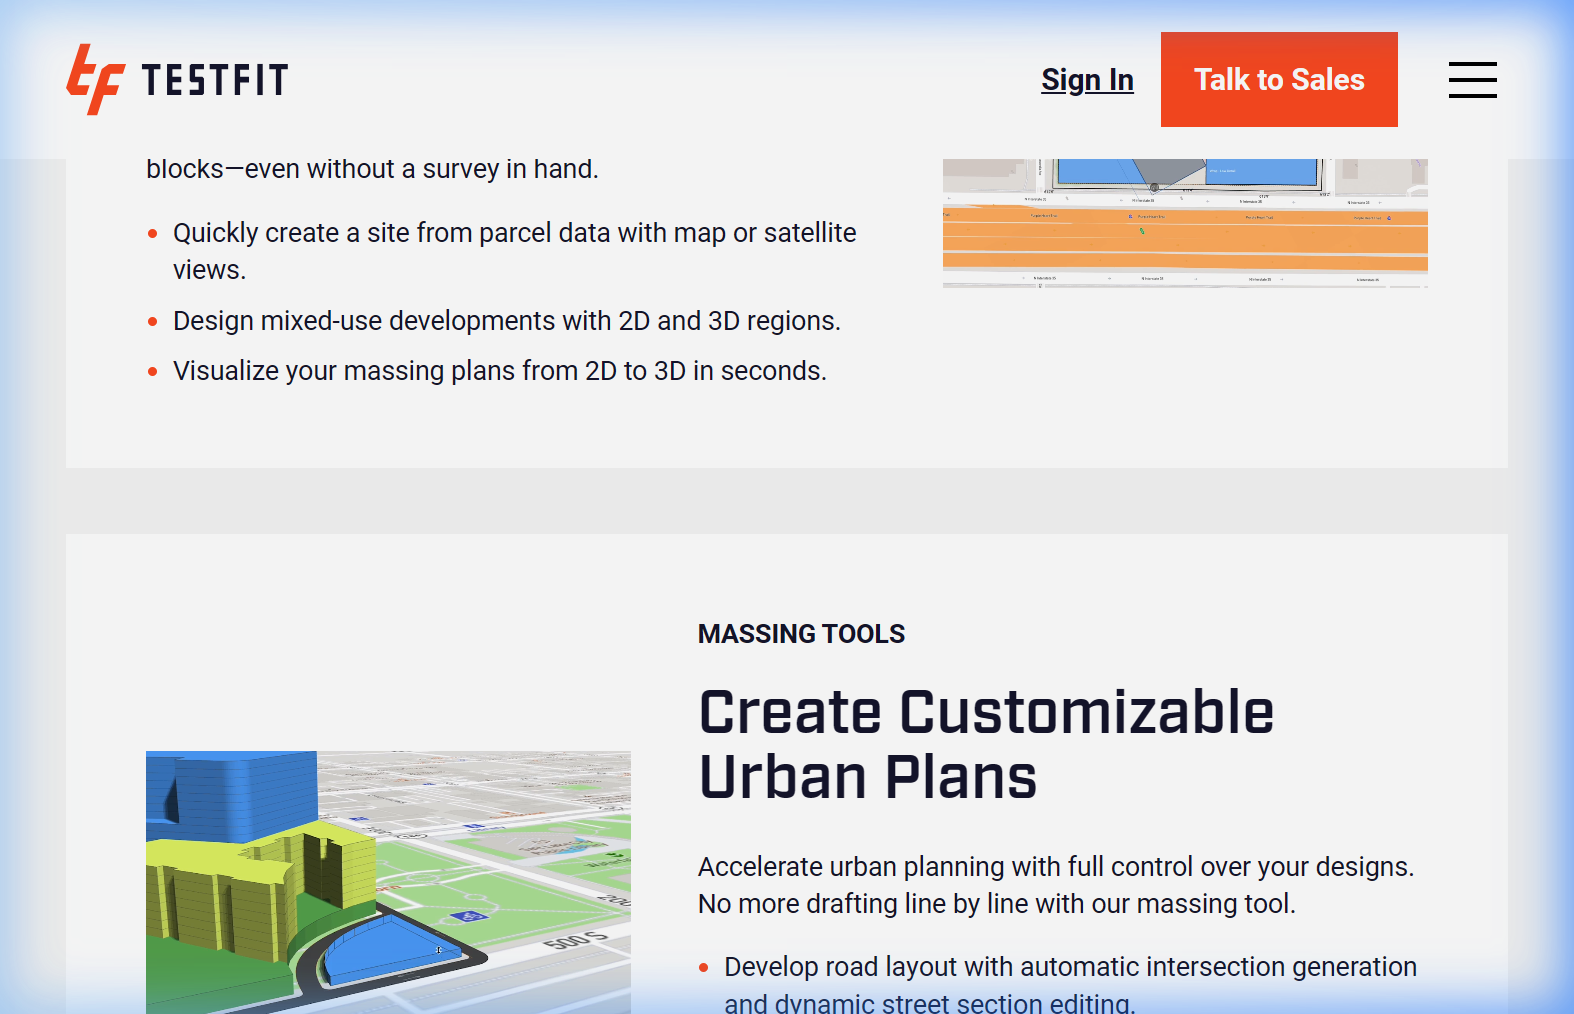
\includegraphics[width=\textwidth]{testfit_massing.png}
      \vspace{0.15cm}
      \begin{center}
        \textcolor{textgray}{\scriptsize Source: testfit.io/product/site-solver}
      \end{center}
    \end{column}
    \begin{column}{0.54\textwidth}
      \vspace{0.2cm}
      \begin{itemize}
        \item[\textcolor{heading}{$\triangleright$}] A \textbf{real estate feasibility platform} for early-stage site planning
        \item[\textcolor{heading}{$\triangleright$}] Generates building layouts under zoning, parking, and financial constraints in seconds
        \item[\textcolor{heading}{$\triangleright$}] Integrates with Revit and AutoCAD for downstream design
      \end{itemize}
      \vspace{0.3cm}
      \textcolor{textgray}{\small Vendor framing (testfit.io):}\\[2pt]
      \textcolor{textwhite}{\small\textit{``Win Profitable Deals.''}}\\[6pt]
      \textcolor{heading}{\small Note the language: the unit of analysis is a \textbf{deal}, not a building or a neighborhood.}
    \end{column}
  \end{columns}
\end{frame}

% ===== SLIDE 3: How It Works =====
\begin{frame}{Design Through Financial and Regulatory Parameters}
  \begin{columns}[T]
    \begin{column}{0.48\textwidth}
      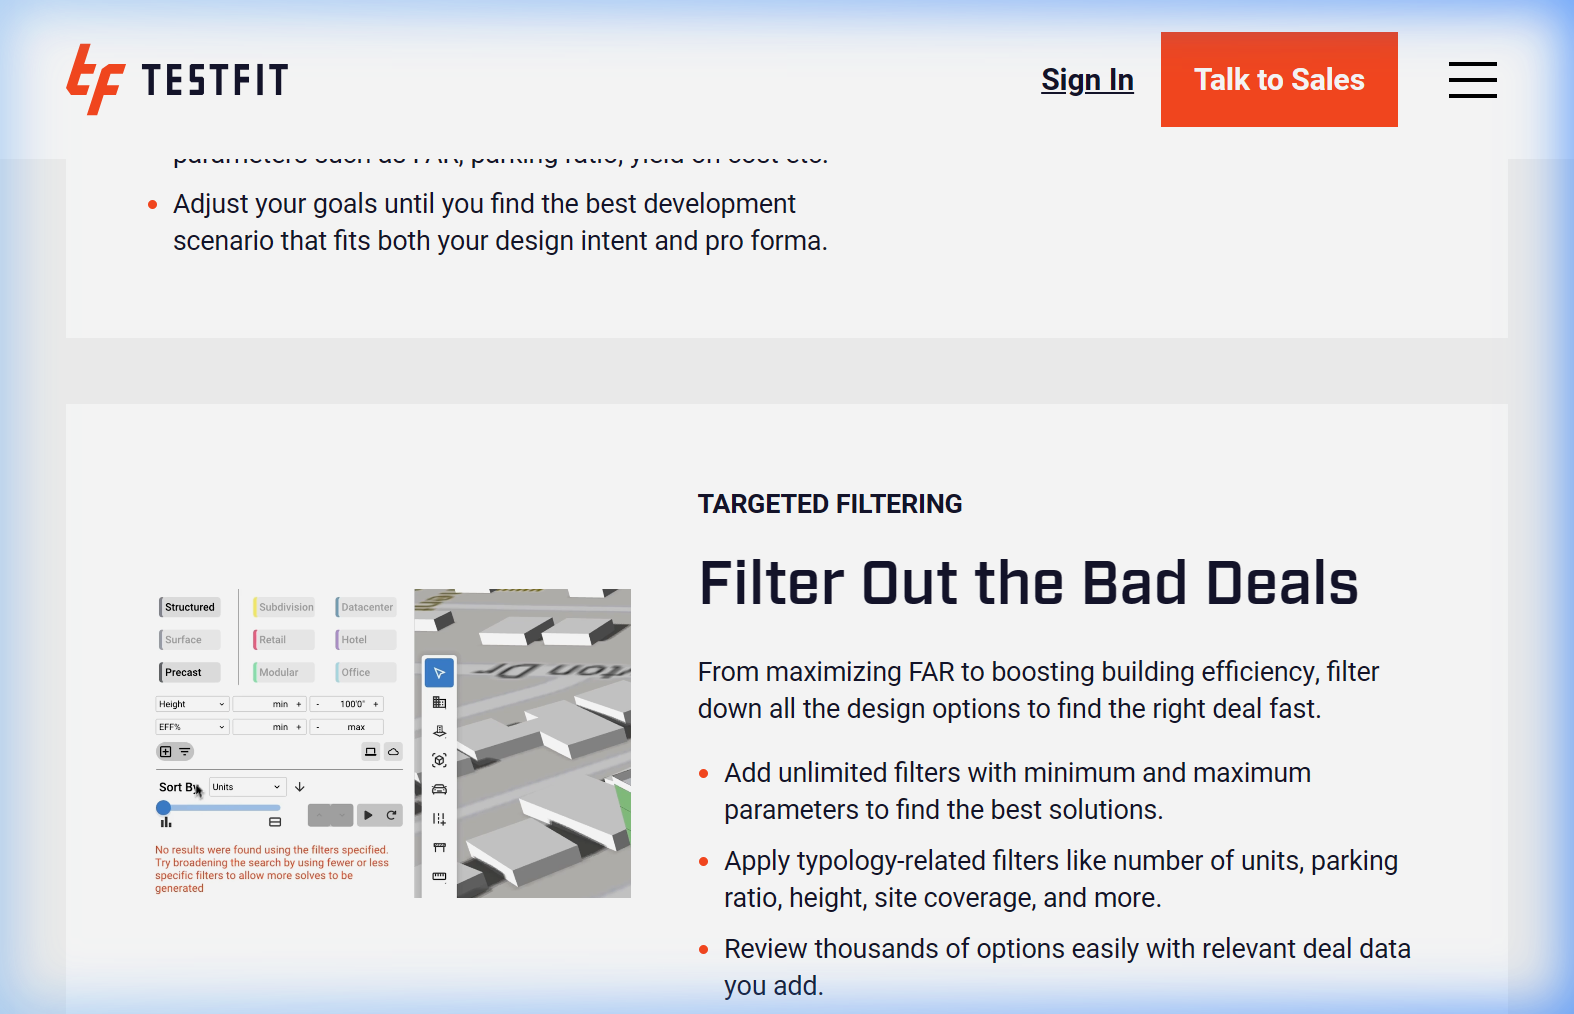
\includegraphics[width=\textwidth]{testfit_deal_filters.png}
      \vspace{0.15cm}
      \begin{center}
        \textcolor{textgray}{\scriptsize Deal filter interface: FAR, height, efficiency, parking ratio}\\
        \textcolor{textgray}{\scriptsize Source: testfit.io/product/deal-evaluation}
      \end{center}
    \end{column}
    \begin{column}{0.48\textwidth}
      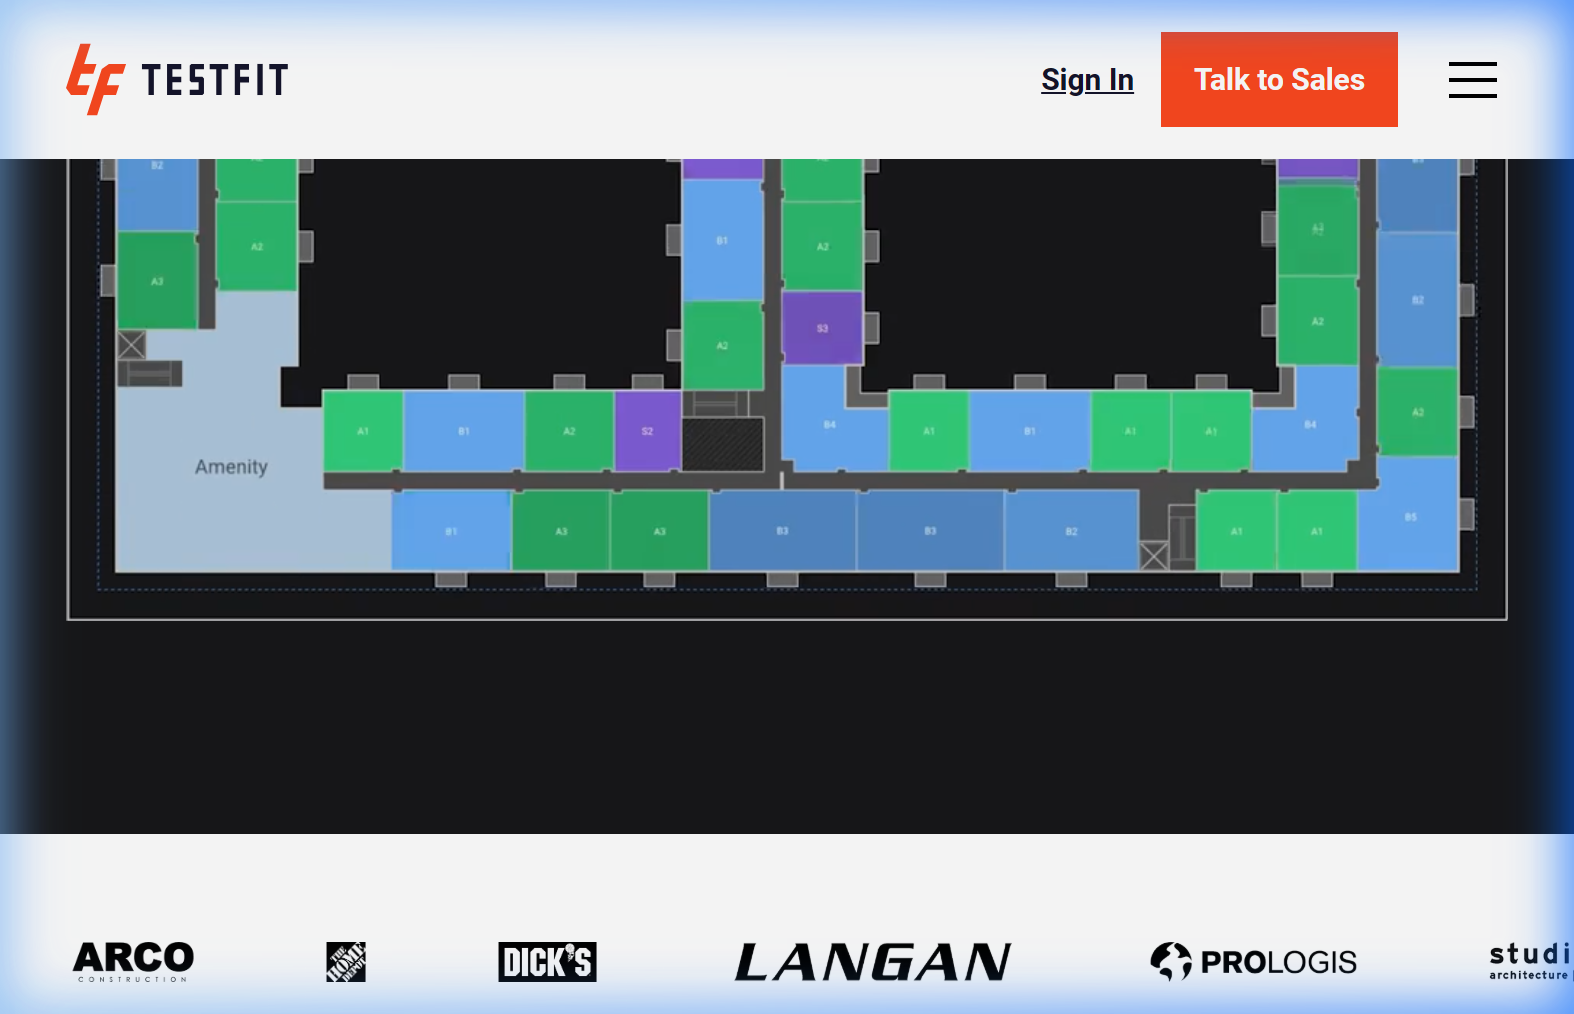
\includegraphics[width=\textwidth]{testfit_plan_view.png}
      \vspace{0.15cm}
      \begin{center}
        \textcolor{textgray}{\scriptsize Algorithmically generated unit layout}\\
        \textcolor{textgray}{\scriptsize Source: testfit.io/product/site-solver}
      \end{center}
    \end{column}
  \end{columns}
  \vspace{0.25cm}
  \begin{center}
    \textcolor{muted}{\small Users adjust yield, FAR, and parking constraints; the algorithm generates the physical form.}
  \end{center}
\end{frame}

% ===== SLIDE 4: What It Optimizes --- and What It Cannot =====
\begin{frame}[shrink=5]{Included and Excluded Values}
  \begin{columns}[T]
    \begin{column}{0.38\textwidth}
      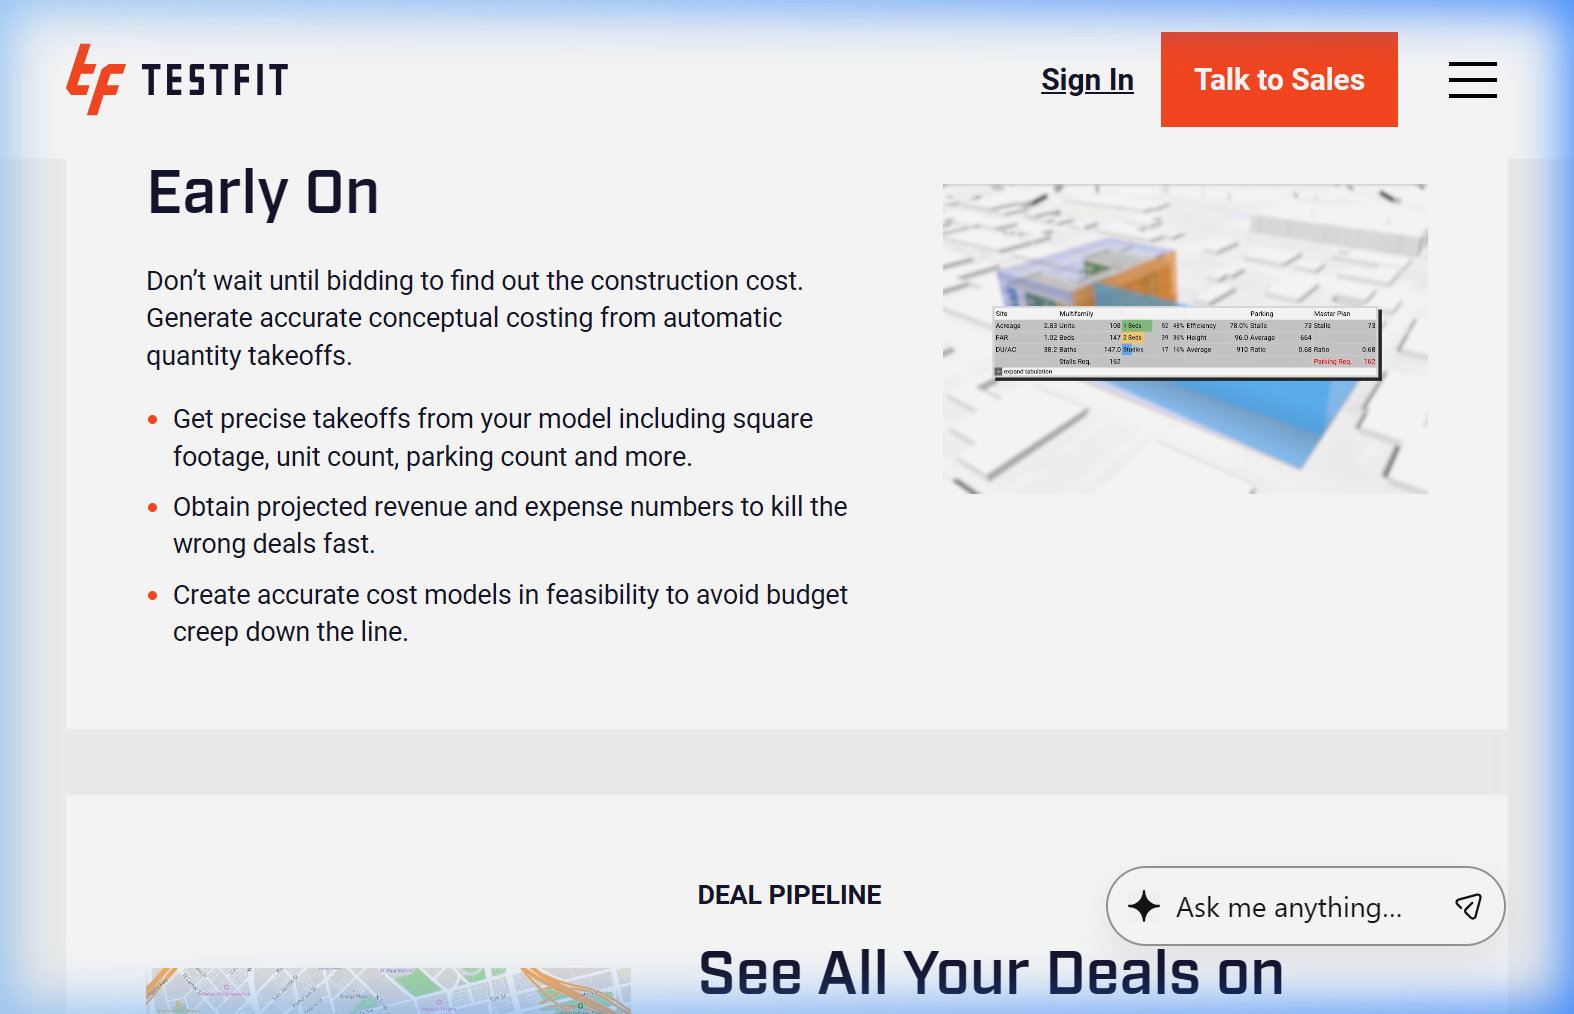
\includegraphics[width=\textwidth,height=0.48\textheight,keepaspectratio]{testfit_quantity_takeoff.png}
      \vspace{0.1cm}
      \begin{center}
        \textcolor{textgray}{\scriptsize Metrics: acreage, FAR, units, efficiency,}\\
        \textcolor{textgray}{\scriptsize height, parking stalls, ratio}\\
        \textcolor{textgray}{\scriptsize Source: testfit.io/product/deal-evaluation}
      \end{center}
    \end{column}
    \begin{column}{0.58\textwidth}
      \textcolor{heading}{\small\textbf{Representable in the software:}}
      \begin{itemize}\setlength{\itemsep}{1pt}
        \item[\textcolor{heading}{\scriptsize$\checkmark$}] {\small Unit count, FAR, building efficiency}
        \item[\textcolor{heading}{\scriptsize$\checkmark$}] {\small Parking ratio, site coverage}
        \item[\textcolor{heading}{\scriptsize$\checkmark$}] {\small Pro forma revenue and cost estimates}
        \item[\textcolor{heading}{\scriptsize$\checkmark$}] {\small Zoning envelope compliance}
      \end{itemize}
      \vspace{0.15cm}
      \textcolor{accent}{\small\textbf{Not primary optimization targets:}}
      \begin{itemize}\setlength{\itemsep}{1pt}
        \item[\textcolor{accent}{\scriptsize$\times$}] {\small Contextual design considerations}
        \item[\textcolor{accent}{\scriptsize$\times$}] {\small Displacement risk or affordability}
        \item[\textcolor{accent}{\scriptsize$\times$}] {\small Community preferences or political feasibility}
        \item[\textcolor{accent}{\scriptsize$\times$}] {\small Environmental or public health impacts}
      \end{itemize}
    \end{column}
  \end{columns}
  \vspace{0.1cm}
  \begin{center}
    \textcolor{accent}{\small\textbf{The question is not whether optimization is useful, but which values}}\\
    \textcolor{accent}{\small\textbf{get encoded and whose objectives the optimization serves.}}
  \end{center}
\end{frame}

% ===== SLIDE 5: Implications for Bargaining Power =====
{
\usebackgroundtemplate{%
  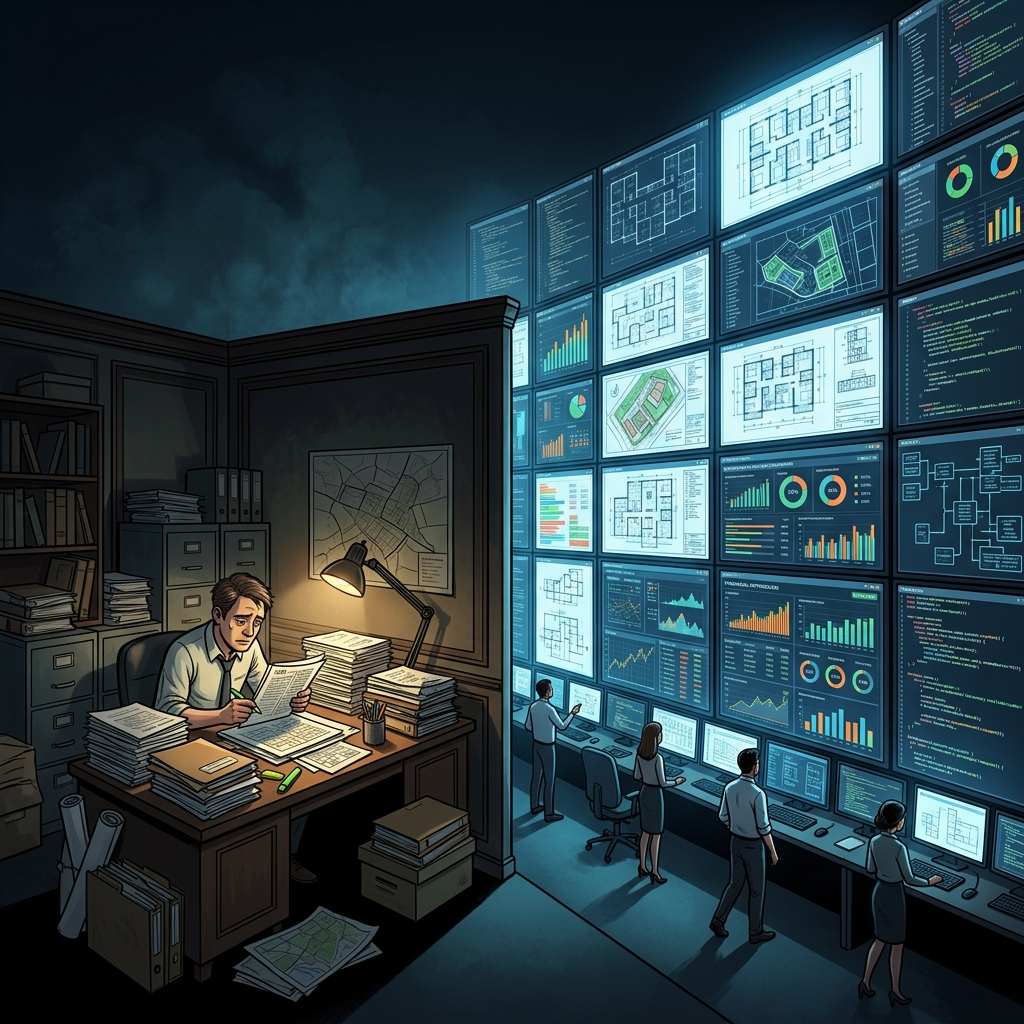
\includegraphics[width=\paperwidth,height=\paperheight]{leverage_asymmetry.png}%
}
\begin{frame}[plain]
  \vspace{0.3cm}
  \hfill
  \colorbox{bgdark!90!black}{%
    \parbox{0.55\textwidth}{\raggedright\vspace{10pt}
      {\large\bfseries\textcolor{heading}{Who Has Access?}}\\[12pt]
      \textcolor{textwhite}{\small
      Developers iterate numerous compliant layouts before a hearing. Reviewing agencies evaluate one submission at a time.}\\[12pt]
      \textcolor{accent}{\small\textbf{Asymmetric modeling capacity can shift bargaining power.}}
    \vspace{10pt}}%
  }
  \hspace{0.2cm}
\end{frame}
}

% ===== SLIDE 6: Closing Question =====
\begin{frame}{}
  \vspace{1.5cm}
  \begin{center}
    {\Large\textcolor{heading}{\textit{When feasibility is evaluated through proprietary,}}}\\[6pt]
    {\Large\textcolor{heading}{\textit{high-speed optimization, which values become}}}\\[6pt]
    {\Large\textcolor{heading}{\textit{easier to represent, and which values}}}\\[6pt]
    {\Large\textcolor{heading}{\textit{become harder to defend?}}}\\[1.2cm]
    \textcolor{textgray}{\small Daniel Hardesty Lewis}\\[2pt]
    \textcolor{textgray}{\small PLAN A6613: AI and the Future of Cities}\\[2pt]
    \textcolor{textgray}{\small Product documentation: testfit.io}
  \end{center}
\end{frame}

\end{document}
